% ====================================================================
%  面向 ML-KEM 解封装实现的时间侧信道泄漏检测研究
%  编译建议：xelatex -> bibtex -> xelatex -> xelatex
% ====================================================================
\documentclass[12pt,a4paper,fontset=none]{ctexart}

\usepackage[top=2.5cm,bottom=2.5cm,left=3cm,right=2.5cm]{geometry}
\usepackage{amsmath,amssymb,mathtools}
\usepackage{graphicx}
\usepackage{subcaption}
\usepackage{booktabs}
\usepackage{multirow}
\usepackage{array}
\usepackage{float}
\usepackage{setspace}
\usepackage{enumitem}
\usepackage{caption}
\usepackage{cite}
\usepackage{algorithm}
\usepackage{algpseudocode}
\usepackage{xcolor}
\usepackage{fancyhdr}
\usepackage{titlesec}
\usepackage[colorlinks=true,linkcolor=black,citecolor=blue,urlcolor=blue]{hyperref}

\setCJKmainfont{Songti SC}[BoldFont={Heiti SC}]
\setCJKsansfont{Heiti SC}
\setCJKmonofont{Heiti SC}
\newCJKfontfamily\papersong{Songti SC}
\newCJKfontfamily\paperhei{Heiti SC}
\newCJKfontfamily\paperkai[
  Path=/System/Library/AssetsV2/com_apple_MobileAsset_Font8/6331c5916c361af1b83fb8b8b76ef2eece20c8eb.asset/AssetData/
]{Kai.ttf}

\graphicspath{{../results/paper_artifacts/}{../results/delay_sweep_run/delay_sweep/}{figures/}}

\pagestyle{fancy}
\fancyhf{}
\fancyhead[L]{\small 面向 ML-KEM 解封装实现的时间侧信道泄漏检测研究}
\fancyhead[R]{\small \thepage}
\renewcommand{\headrulewidth}{0.4pt}
\setlength{\headheight}{14pt}

\onehalfspacing
\captionsetup{font=small,labelfont=bf,skip=6pt}
\setlist{nosep,leftmargin=2em}
\renewcommand{\algorithmicrequire}{\textbf{输入:}}
\renewcommand{\algorithmicensure}{\textbf{输出:}}
\floatname{algorithm}{算法}

\titleformat{\section}{\large\bfseries}{\thesection}{1em}{}
\titleformat{\subsection}{\normalsize\bfseries}{\thesubsection}{1em}{}

\newcommand{\mlkem}{ML-KEM}
\newcommand{\balacc}{\mathrm{BalAcc}}

\newcommand{\makepapercover}{
  \begin{titlepage}
    \thispagestyle{empty}
    \centering
    \vspace*{4.2cm}
    {\paperhei\bfseries\zihao{2}
      面向 ML-KEM 解封装实现的\\[1.0em]
      时间侧信道泄漏检测研究\par}
    \vspace{1.2cm}
    \rule{0.62\textwidth}{0.5pt}
    \vspace{2.6cm}

    {\papersong\zihao{4}
    \begin{tabular}{>{\raggedleft\arraybackslash}p{4.0cm} p{5.4cm}}
      课\quad 程\quad 名\quad 称： & 量子计算与后量子密码 \\[1.1em]
      学\quad 生\quad 姓\quad 名： & 寇得一 \\[1.1em]
      学\qquad\qquad 号： & 2023211545 \\[1.1em]
      学\qquad\qquad 院： & 网络空间安全学院 \\[1.1em]
      专\qquad\qquad 业： & 信息安全 \\[1.1em]
      指\quad 导\quad 教\quad 师： & 窦钊 \\
    \end{tabular}
    \par}

    \vfill
    {\papersong\zihao{3} 2026 年 5 月\par}
    \vspace*{2.0cm}
  \end{titlepage}
}

\begin{document}

\hypersetup{pageanchor=false}
\makepapercover
\clearpage
\hypersetup{pageanchor=true}
\pagenumbering{Roman}

\thispagestyle{empty}
\begin{center}
  {\paperkai\zihao{3} 摘\quad 要}
\end{center}
\vspace{0.8em}
{\paperkai
随着后量子密码标准化推进，ML-KEM 已成为密钥封装机制的重要部署对象。然而，算法
层面的标准化并不等同于具体软件实现的侧信道安全。本文面向 \texttt{pqcrypto} 库中的
ML-KEM-512、ML-KEM-768 和 ML-KEM-1024 解封装实现，构建了一套基于统计检验与机器
学习的软件时间侧信道泄漏筛查流程。实验比较有效密文与四类同长度无效密文输入，提取
13维时间统计特征，并结合 Welch's $t$ 检验、KS 检验、Cohen's $d$、逻辑回归、线性
SVM、随机森林和梯度提升树进行多证据判定。

在5轮独立重复、3个参数集和4种无效密文策略构成的60次完整实验中，固定延迟正对照均
能被稳定识别，说明检测管线具备识别已知时间信号的能力；真实场景下最佳模型平衡准确率
均值为0.5134，60次实验均未触发泄漏判定。结果表明，在本文的软件计时条件、输入模型
和被测实现版本下，未检测到 ML-KEM 解封装过程对有效密文与无效密文表现出稳定、可区分
的时间侧信道泄漏。该结论属于实现级筛查结论，不构成形式化侧信道安全证明。本文全部
采集脚本、原始数据与分析代码已开源：\url{https://github.com/AndrewAccuracy/PostQuantum}。

\vspace{0.8em}
\noindent{\paperkai 关键词：}后量子密码；ML-KEM；时间侧信道；机器学习；泄漏检测
\par}

\newpage
\tableofcontents
\newpage
\pagenumbering{arabic}

\section{引言}
\label{sec:intro}

\subsection{研究背景}

公钥密码体制是现代网络安全基础设施的核心组成部分，广泛用于密钥协商、身份认证、
软件签名和安全通信协议。RSA、Diffie-Hellman 和椭圆曲线密码等经典方案的安全性
主要建立在大整数分解和离散对数问题的计算困难性之上。Shor 在1994年提出的量子
算法表明，具备足够规模和纠错能力的量子计算机能够在多项式时间内求解这两类问题
~\cite{Shor1994}。因此，即便大规模通用量子计算机尚未实用化，密码系统也需要提前
迁移到能够抵抗量子攻击的后量子密码算法。

这种迁移需求具有明显的前置性。一方面，公钥密码算法深嵌在 TLS、VPN、软件供应链、
身份认证和长期数据保护等场景中，协议升级、软硬件适配和互操作测试都需要较长周期；
另一方面，部分长期保密数据可能面临``先收集、后解密''风险，即攻击者现在保存加密
通信内容，等待未来量子计算能力成熟后再尝试解密。因而，后量子密码的研究不只是
算法竞赛意义上的理论问题，也直接关系到现有系统能否平滑完成密码迁移。

NIST 自2016年启动后量子密码标准化进程，并于2024年发布首批后量子密码标准。其中
FIPS 203 将 CRYSTALS-Kyber 标准化为 Module-Lattice-Based Key-Encapsulation
Mechanism，即 ML-KEM~\cite{FIPS203,Kyber2021}。本文依据 FIPS 203 正式发布版
展开实验，不单独分析后续 errata 对实现行为的影响。ML-KEM 基于模格误差学习
（Module Learning With Errors，MLWE）问题，提供 ML-KEM-512、ML-KEM-768 和
ML-KEM-1024 三组参数，分别对应不同安全级别和性能开销。

在实际协议中，KEM 通常用于在不安全信道上协商共享密钥，再由对称密码承担后续数据
加密任务。与传统公钥加密相比，KEM 的接口更贴近现代混合密钥交换协议，也更适合作为
后量子迁移中的基础组件。ML-KEM 的三个参数集在安全级别、密钥长度、密文长度和运行
开销之间提供不同折中；因此，仅考察单一参数集不足以反映部署时可能遇到的实现行为，
有必要在全参数集上进行横向测试。

然而，算法标准化解决的是规范层面的安全问题，并不能自动保证具体实现没有侧信道
泄漏。Kocher 的时序攻击工作最早系统性说明了公钥密码操作的执行时间可能泄露私钥
信息~\cite{Kocher1996}；Bernstein 随后展示了缓存状态也可能形成可利用的时间差异
~\cite{Bernstein2005}。对于后量子 KEM 而言，解封装阶段同时接收攻击者可控密文并
使用私钥，是实现安全分析中的重点环节。已有研究表明，CCA 安全格基 KEM 中的
Fujisaki-Okamoto 变换和重加密验证步骤可能成为功耗或电磁侧信道分析的重要目标
~\cite{Ravi2020,Ueno2022}。因此，对 ML-KEM 实现开展可复现的泄漏检测具有直接的
工程意义。

从工程评估角度看，侧信道问题往往出现在规范与实现之间的缝隙中。规范可以要求解封装
接口在验证失败时仍输出伪随机共享密钥，却很难完全限定编译器优化、底层算术指令、
内存层次结构和运行时环境带来的微小时间差异。对于软件库使用者而言，最先需要回答的
问题通常不是能否立即构造密钥恢复攻击，而是某一实现是否已经表现出可稳定观测的
异常时间行为。本文正是在这一层面上展开：把端到端解封装时间作为可观测信道，对
有效密文与多类同长度无效密文进行可复现筛查。

\subsection{研究目的与问题提出}
\label{sec:purpose}

本文的研究目的，是面向 ML-KEM 解封装这一实现安全敏感环节，建立一套可复现、可量化、
可解释的软件时间侧信道泄漏筛查方法。本文不以构造完整密钥恢复攻击为目标，也不试图
证明某一实现具备形式化侧信道安全性，而是关注攻击者可控密文输入是否会使解封装过程
表现出稳定、可检测、可进一步分析的执行时间差异。

本文选择解封装作为观测对象，主要基于两点考虑。首先，解封装接口同时处理私钥和外部
输入密文，攻击者可以反复提交选择密文并观察返回行为，是 KEM 实现中最接近选择密文
攻击模型的接口。其次，ML-KEM 的解封装过程包含解密、重加密、密文比较和失败路径
密钥派生等步骤；这些步骤在规范上应避免泄露成功或失败路径差异，但在具体软件实现中
仍可能受到分支、内存访问、算术指令延迟和异常处理路径的影响。因此，比较有效密文与
无效密文的端到端时间分布，是发现实现级异常行为的一种直接入口。

围绕上述目的，本文主要回答以下研究问题：

\begin{description}[leftmargin=3.5em,labelsep=0.6em]
  \item[RQ1] 在 \texttt{pqcrypto} 库提供的 ML-KEM-512、ML-KEM-768 和 ML-KEM-1024
        解封装实现中，有效密文与无效密文之间是否存在可由统计检验识别的执行时间差异？
  \item[RQ2] 在多维时间统计特征下，机器学习分类器能否在未见过的基础密文组上稳定
        区分有效密文与无效密文？
  \item[RQ3] 不同参数集和不同无效密文构造策略是否会改变泄漏检测结果？
  \item[RQ4] 在软件计时噪声存在的条件下，本文检测管线能否识别已知人为时间信号，
        其灵敏度边界大致处于什么量级？
\end{description}

通过上述问题，本文希望给出一个边界清晰的实现级判断：若检测到稳定信号，则说明被测
实现需要进一步侧信道审计；若未检测到稳定信号，则只能说明在本文平台、输入模型和计时
方法下没有发现可区分泄漏，而不能推出算法或实现的绝对侧信道安全。

上述问题的提出基于两个事实。第一，ML-KEM 已进入标准化和部署阶段，FIPS 203 对
算法接口、参数和正确性给出规范，但实现仍需接受独立的侧信道评估~\cite{FIPS203}。
第二，传统测试向量泄漏评估（TVLA）强调通过统计检验发现两类输入之间的泄漏信号
~\cite{Becker2013}，而机器学习分类器能够从多维特征组合中发现非线性或非均值差异。
因此，本文将参数检验、非参数检验、效应量和机器学习判别能力结合起来，形成多证据
交叉验证的实现级检测方法。

\subsection{主要贡献}

本文的主要贡献如下：

\begin{enumerate}
  \item 面向 ML-KEM 解封装实现，构建了一套可复现的软件时间侧信道泄漏筛查框架，
        覆盖 ML-KEM-512、ML-KEM-768 和 ML-KEM-1024 三个参数集，并支持多轮重复实验
        与自动化结果分析。
  \item 设计了四类同长度无效密文输入模型，包括单比特扰动、字节翻转、伪随机密文和
        全零密文，用于从最小扰动、局部破坏、随机无效输入和极端结构化输入等角度考察
        解封装时间行为。
  \item 结合统计显著性、效应量和机器学习可分性建立多证据泄漏判定方法，并通过分组
        交叉验证降低同一基础密文组带来的记忆性数据泄漏风险。
  \item 引入固定延迟正对照和延迟灵敏度扫描，验证检测管线对已知时间信号的识别能力，
        从而提高负检测结论的可信度。
  \item 基于5轮独立重复、3个参数集和4种无效密文策略的60次完整实验，给出被测
        \texttt{pqcrypto} ML-KEM 解封装实现的软件时间泄漏筛查结果，并明确说明该结果
        的适用边界。
\end{enumerate}

本文其余部分安排如下：第~\ref{sec:related} 节回顾时间侧信道、格基 KEM 侧信道和
机器学习辅助泄漏检测相关研究；第~\ref{sec:background} 节介绍 ML-KEM 参数集、
统计检验与分组机器学习评估基础；第~\ref{sec:design} 节说明实验对象、威胁模型、
无效密文策略和判定规则；第~\ref{sec:results} 节给出实验结果与灵敏度分析；
第~\ref{sec:discussion} 节讨论结果解释、局限性和可复现性；最后总结本文结论。

\section{相关工作}
\label{sec:related}

\subsection{后量子标准化与 ML-KEM 实现评估}

后量子密码标准化的核心目标，是在量子计算威胁下为现有公钥密码基础设施提供可替换的
算法组件。NIST 标准化过程从安全性、性能、密钥与密文规模、实现复杂度和部署可行性等
方面综合评估候选算法，最终将 CRYSTALS-Kyber 标准化为 ML-KEM~\cite{FIPS203,Kyber2021}。
从部署角度看，标准文本给出了算法接口、参数集、编码方式和正确性要求，为不同实现
之间的互操作奠定基础。

但是，标准化并不等价于所有实现都天然满足常数时间或侧信道安全要求。ML-KEM 的实现
可能来自参考代码、优化汇编、语言绑定或第三方密码库，不同实现会受到编译器、处理器
微架构和运行时系统的共同影响。即使两个实现遵循同一算法规范，其内存访问模式、算术
指令选择和错误处理路径也可能存在差异。因此，在算法进入工程部署阶段之后，独立的
实现级测试成为标准化工作之外的必要补充。

本文使用的 \texttt{pqcrypto} 绑定属于应用开发者较容易接触到的软件接口。对这类库
进行黑盒端到端计时测试，不能替代源码审计或硬件侧信道评估，但可以帮助开发者快速
判断常见调用方式下是否出现明显可分辨的时间异常。与仅关注单一参数集的测试相比，
全参数集实验能够进一步观察安全级别提升和数据规模增大是否改变时间行为。

\subsection{时间侧信道与实现安全}

时间侧信道攻击的核心思想是通过观测程序运行时间推断秘密相关信息。Kocher 证明了
不同私钥比特引发的模幂运算路径差异可以通过大量计时观测恢复~\cite{Kocher1996}。
后续远程计时研究进一步说明，即使通过网络进行测量，时序差异仍可能在现实环境下被
利用~\cite{Brumley2005}。Bernstein 对 AES 的缓存时序攻击则表明，侧信道
并不只来自显式分支，内存访问和缓存命中状态同样可能泄露信息~\cite{Bernstein2005}。

软件时间差异的来源较为复杂。除秘密相关分支外，表查找、缓存未命中、数据相关乘除法、
异常处理、内存分配、解释器开销和操作系统调度都可能改变单次调用时间。对于密码实现
而言，常数时间编程通常要求控制流和内存访问不依赖秘密数据，但在高级语言绑定和通用
操作系统环境中，调用边界之外的噪声同样会进入观测结果。因此，端到端软件计时既有
部署相关性，也需要通过重复采样、随机化采集顺序和对照实验降低误判风险。

这些研究推动了常数时间编程和实现级安全评估的发展。对于后量子密码算法，虽然其
数学困难性不同于 RSA 和椭圆曲线密码，但底层软件仍运行在相同的处理器、缓存和
操作系统之上，因此同样需要关注输入相关的执行时间差异。本文将执行时间作为可观测
信道，关注攻击者可控输入是否会在 ML-KEM 解封装实现中诱发稳定的时间差异。

\subsection{泄漏检测与统计评估方法}

侧信道评估中常见的一类方法是测试向量泄漏评估（TVLA）。TVLA 通常构造两类输入或
中间状态，通过统计检验判断观测轨迹是否存在显著差异~\cite{Becker2013}。其优点是
不需要完整攻击流程，也不需要预先知道泄漏模型，适合作为实现进入深入审计前的筛查
工具。其局限也很明确：统计显著只能说明观测分布不同，并不自动说明差异可以用于密钥
恢复；反过来，未通过某一组测试也不能证明实现不存在其他形式的泄漏。

在软件计时场景下，样本分布通常带有长尾和异方差特征。单纯比较均值容易遗漏分布形状
变化，单纯依赖 $p$ 值又可能把样本量带来的极小差异误读为实践风险。因此，本文借鉴
TVLA 的两类输入思想，以 Welch's $t$ 检验~\cite{Welch1947}、KS 检验和 Cohen's $d$
效应量~\cite{Cohen1988} 作为正文中的主要统计证据，并在自动化报告中保留
Mann-Whitney $U$ 检验~\cite{Mann1947} 作为非参数辅助诊断。

此外，泄漏检测本身也需要对误报和漏报保持谨慎。若采集顺序固定，系统负载或温度变化
可能被误认为标签差异；若同一基础密文派生出的样本同时出现在训练集和测试集，分类器
可能记住密文组而不是学习泄漏信号。本文在实验设计中引入随机打乱、分组交叉验证、
多轮重复、固定延迟正对照和延迟灵敏度扫描，目的就是让负检测结论具有更清楚的边界。

\subsection{格基 KEM 的侧信道研究}

CRYSTALS-Kyber/ML-KEM 属于格基 KEM，其解封装过程包含解密、重加密、密文比较和
失败路径密钥派生等步骤。Ravi 等人从通用角度研究了 CCA 安全格基 PKE/KEM 的侧信道
问题，指出若实现泄露解封装成功与失败路径差异，可能为选择密文攻击提供入口
~\cite{Ravi2020}。Ueno 等人提出``重加密诅咒''，展示 FO 变换中的重加密步骤在
功耗与电磁信道下具有泛化的攻击面~\cite{Ueno2022}。Primas 等人则从单轨迹功耗
分析角度说明，即便格密码实现采用一定防护，细粒度实现特征仍可能被分析利用
~\cite{Primas2017}。

这些工作说明，格基 KEM 的实现安全并不只取决于底层困难问题。特别是在 CCA 安全变换
下，解封装需要先根据私钥处理输入密文，再通过重加密或比较步骤决定最终共享密钥的
来源；若成功路径与失败路径在时间、功耗或电磁轨迹上可区分，攻击者就可能获得超出
标准接口的额外信息。因此，有效密文与无效密文的对照测试是 KEM 实现评估中的自然
实验设置。本文使用同长度无效密文，正是为了尽量排除长度错误带来的显式异常路径，
把关注点集中在内容差异是否影响正常解封装流程。

与功耗和电磁分析相比，软件计时实验的攻击门槛更低，但信噪比也更差，因此本文将其
定位为早期筛查方法，而非完整攻击方法。检测到信号说明实现值得进一步审计；未检测到
信号则只能说明当前条件下未发现可区分差异。

值得特别关注的是，KyberSlash 工作报告了 Kyber/ML-KEM 多个实现（包括参考实现）中
确实存在的密钥相关时序泄漏：在 \texttt{poly\_tomsg} 等模块化压缩步骤中，对模数
$q$ 的变长除法运算耗时与中间值相关，攻击者可在 Cortex-A7 和 Cortex-M4 等平台上
通过该时序差异在数分钟到数小时内恢复密钥~\cite{Bernstein2025}。这一案例表明，
ML-KEM 的时间侧信道泄漏并非纯理论假设，而是已在真实实现中被发现并修复的问题。
该工作同时提出基于 Valgrind 的指令级污点分析方法，用于在源码层面定位变长时间
操作。本文与之的主要区别在于观测粒度：KyberSlash 类工作针对单条指令或单个算术
运算的执行时间，而本文从输入（有效/无效密文）到端到端解封装耗时这一更粗粒度的
黑盒视角出发，因此二者在检测能力和适用阶段上是互补的。

\subsection{机器学习辅助泄漏检测}

机器学习方法已广泛用于侧信道分析中的模板攻击和特征识别。Lerman 等人比较了随机
森林、支持向量机和 $k$ 近邻等模型在功耗分析中的表现~\cite{Lerman2015}；Cagli
等人将卷积神经网络用于带有抖动对抗措施的功耗轨迹，展示了深度学习方法对复杂轨迹
错位的适应能力~\cite{Cagli2017}。但深度模型通常需要大量轨迹和更高训练成本，且
可解释性较弱。

本文面向小样本、端到端、筛查型的软件计时任务，因此选择逻辑回归、线性 SVM、随机
森林和直方图梯度提升树作为检测模型。这些模型既能覆盖线性与非线性判别，又便于与
统计检验和特征重要性分析结合。本文将机器学习分类结果作为统计检验之外的补充证据，
而不是以模型准确率替代传统泄漏评估；模型置换检验仅作为输出报告中的辅助诊断，不进入
正文泄漏判定条件。

需要注意的是，机器学习方法用于泄漏检测时尤其容易受到数据划分方式影响。如果训练集
和测试集共享同一基础密文组，模型可能学习到某些偶然的组内计时特征，从而给出虚高的
测试准确率。另一方面，在没有真实信号的数据上，复杂模型也可能通过过拟合产生局部
波动。因此，本文使用分组交叉验证约束同一基础密文组不会同时出现在训练集和测试集，
并将模型准确率与统计检验、效应量和正对照结果一起解释。这样做的目标不是
追求最高分类性能，而是让机器学习结果成为更稳健的泄漏筛查证据。

\section{理论基础}
\label{sec:background}

\subsection{ML-KEM 参数集}

ML-KEM 是一种密钥封装机制，包含密钥生成、封装和解封装三个接口。其安全性基于模格
误差学习问题，底层多项式环通常记为
$R_q=\mathbb{Z}_q[X]/(X^{256}+1)$，其中 $q=3329$。三个参数集的主要差异在于模块
维度 $k$ 和压缩参数，进而影响公钥、密文、私钥大小和计算开销。表~\ref{tab:mlkem}
列出 FIPS 203 中与本文实验相关的主要参数~\cite{FIPS203}。

\begin{table}[H]
  \centering
  \caption{ML-KEM 三个参数集的接口规模}
  \label{tab:mlkem}
  \begin{tabular}{lrrrr}
    \toprule
    参数集 & NIST 安全级别 & 公钥大小（B） & 密文大小（B） & 私钥大小（B） \\
    \midrule
    ML-KEM-512  & 1 & 800   & 768  & 1632 \\
    ML-KEM-768  & 3 & 1184  & 1088 & 2400 \\
    ML-KEM-1024 & 5 & 1568  & 1568 & 3168 \\
    \bottomrule
  \end{tabular}
\end{table}

本文重点测量解封装阶段。该阶段输入私钥和外部密文，输出共享密钥。若密文验证失败，
实现应返回由私钥中随机种子和输入密文派生的伪随机值，而不是泄露失败路径的内部
状态。理想情况下，有效密文和无效密文不应在可观测时间上形成稳定差异。

\subsection{统计检验与效应量}

设有效密文样本的聚合均值时间为 $\{x_i\}_{i=1}^{n_0}$，无效密文样本为
$\{y_i\}_{i=1}^{n_1}$。Welch's $t$ 检验用于判断两组均值是否存在显著差异，且不要求
两组方差相等~\cite{Welch1947}：
\begin{equation}
  t_W=\frac{\bar{x}-\bar{y}}
  {\sqrt{s_x^2/n_0+s_y^2/n_1}} .
  \label{eq:welch}
\end{equation}
在本文中，Welch's $t$ 检验主要用于判断两类输入的平均解封装时间是否存在显著差异。
Mann-Whitney $U$ 检验不依赖正态分布假设，更适合长尾计时数据~\cite{Mann1947}。
KS 检验比较两组经验分布函数的最大距离，可检测均值之外的整体分布形状变化。
Cohen's $d$ 用于衡量差异的实践大小~\cite{Cohen1988}：
\begin{equation}
  d=\frac{\bar{y}-\bar{x}}
  {\sqrt{(s_x^2+s_y^2)/2}} .
  \label{eq:cohen}
\end{equation}
其中，KS 检验用于判断两类时间分布整体形态是否不同；Cohen's $d$ 用于判断差异是否
具有实际效应，而不只是统计显著。
本文将 $p<0.01$ 作为主要统计显著性阈值，将 $|d|\ge 0.2$ 作为可解释效应的最低
阈值。

\subsection{分组机器学习评估}

在分类检测中，特征向量由每条聚合轨迹的13维统计量构成，标签表示有效密文或无效
密文。本文使用平衡准确率作为主要指标：
\begin{equation}
  \balacc=\frac{1}{2}\left(\frac{TP}{TP+FN}+\frac{TN}{TN+FP}\right).
  \label{eq:balacc}
\end{equation}
在本文中，平衡准确率用于衡量模型对有效密文和无效密文的泛化区分能力。
两类样本数量相等时，随机猜测的期望平衡准确率为0.5。为避免模型记住同一基础密文组
的偶然计时特征，本文使用 \texttt{GroupShuffleSplit}，要求同一 \texttt{group\_id}
下的有效样本和无效样本始终同时位于训练集或测试集一侧。随机森林使用 Breiman 的
集成树模型~\cite{Breiman2001}，梯度提升树参考提升树的逐步残差拟合思想~\cite{Friedman2001}，
模型实现基于 scikit-learn~\cite{Pedregosa2011}。

\clearpage
\section{实验设计与实现}
\label{sec:design}

\subsection{总体技术路线}

本文的检测流程由输入构造、计时采集、特征提取、统计检验、机器学习评估和泄漏判定
六个部分组成。整体架构如图~\ref{fig:overall_architecture} 所示：首先针对三个
ML-KEM 参数集生成有效密文，并按照四种策略构造同长度无效密文；随后在真实场景和
固定延迟正对照场景下采集解封装时间；最后将原始计时聚合为统计特征，并用多种统计
检验和分类模型交叉判断是否存在稳定可区分的时间差异。

\begin{figure}[H]
  \centering
  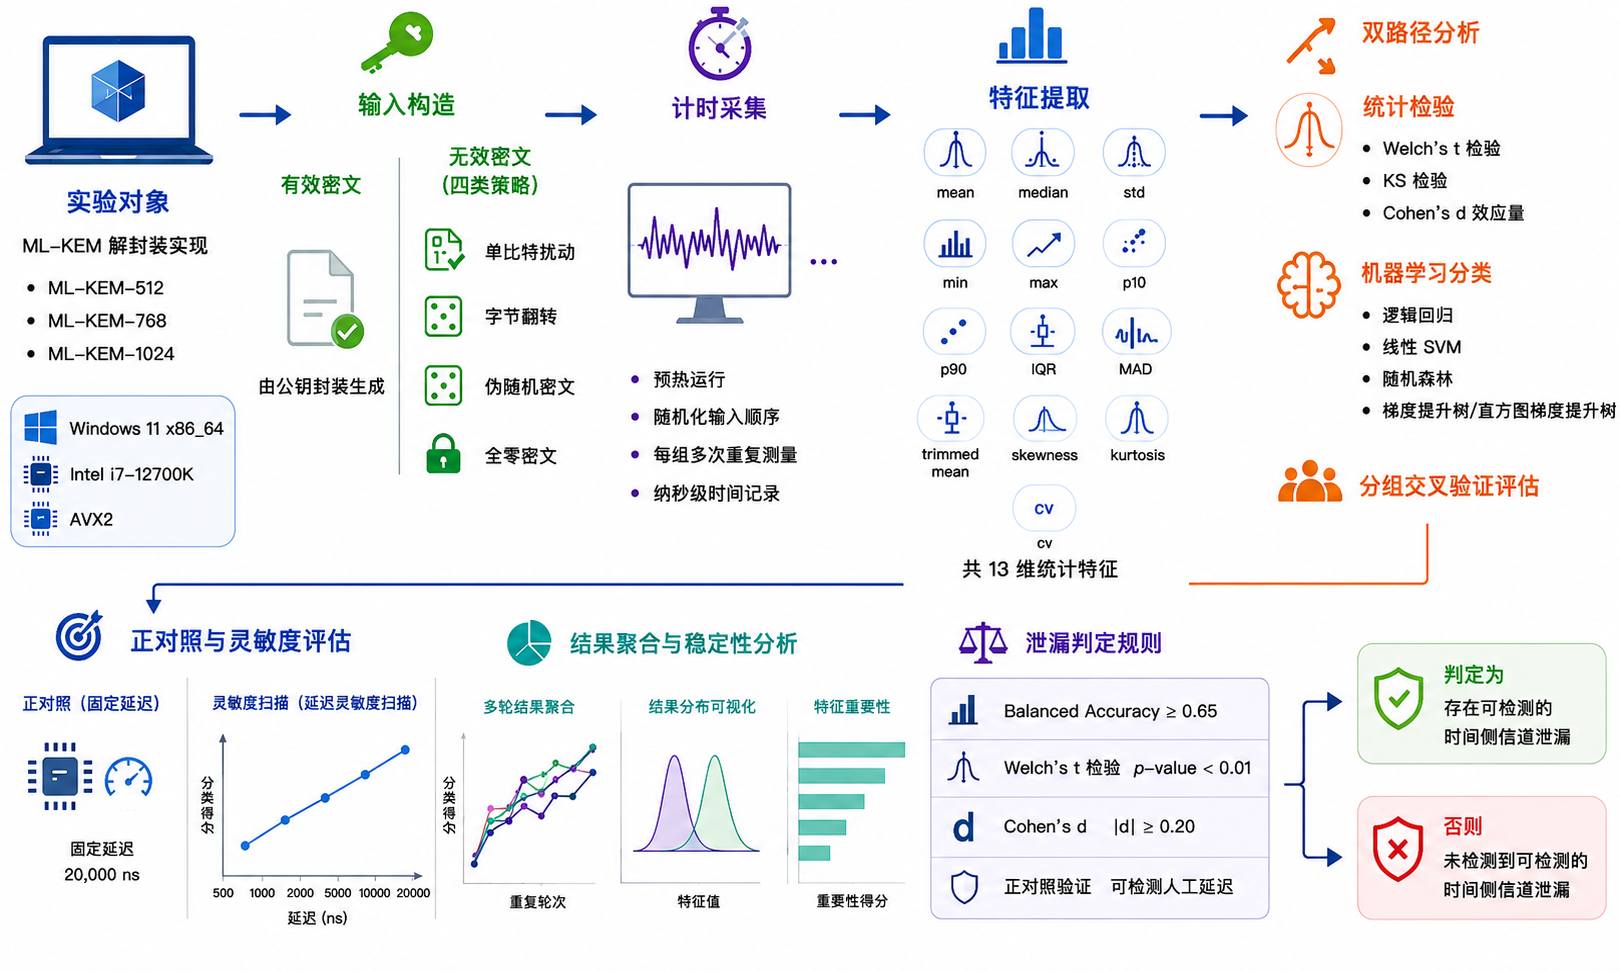
\includegraphics[width=\textwidth]{overall_architecture.png}
  \caption{ML-KEM 解封装时间侧信道泄漏检测整体架构}
  \label{fig:overall_architecture}
\end{figure}

\subsection{威胁模型与观测模型}
\label{sec:threat-model}

本文考虑的攻击者是与被测程序运行在同一台机器上的本地、协同驻留进程。该攻击者
具备类似 CCA 模型中的选择密文能力：可以构造任意同长度密文并提交给目标实现的
解封装接口，但不能访问私钥或其内部状态。与标准 CCA 安全模型不同的是，本文攻击者
额外具备本地高精度时间侧信道观测能力；其通过被测进程自身提供的高精度计时接口
（Python \texttt{time.perf\_counter\_ns}）获取每次解封装调用的墙钟时间，不依赖
缓存探测、性能计数器或功耗/电磁探针等更强的旁路观测手段。

观测模型上，本文不直接使用单次调用的原始计时，而是将连续 $R=50$ 次解封装的耗时
聚合为均值等13维统计特征，再据此判断有效密文与无效密文是否可区分。这一设置对应
攻击者可以多次重放同一密文并进行统计平均的场景，但不对应一次性观测、网络传输
延迟主导或攻击者只能获得粗粒度计时（如毫秒级）的更弱场景——在后两种场景下，本文
方法提供的灵敏度上界会进一步劣化。本文的判定结论应在该观测模型下理解：若在
本地、可重复采样、纳秒级精度的有利条件下仍未检测到稳定差异，则在更弱的观测条件
（如 Brumley 和 Boneh 讨论的远程网络计时~\cite{Brumley2005}）下检测到差异的可能性
只会更低，而不会更高。

\subsection{实验对象与运行环境}

本文实验对象为 Python \texttt{pqcrypto==0.3.4} 包提供的 ML-KEM 三个参数集绑定
（512、768 和1024）。
正式论文数据来自 Windows 11 x86\_64 平台，软件环境
如表~\ref{tab:env} 所示。

\begin{table}[H]
  \centering
  \caption{正式实验运行环境}
  \label{tab:env}
  \begin{tabular}{>{\raggedright\arraybackslash}p{0.43\textwidth}
                  >{\raggedright\arraybackslash}p{0.47\textwidth}}
    \toprule
    项目 & 配置 \\
    \midrule
    CPU & Intel Core i7-12700K（支持 AVX2） \\
    操作系统 & Windows 11 x86\_64（10.0.26200） \\
    Python & 3.12.12（Anaconda 发行版） \\
    ML-KEM 实现 & \texttt{ml\_kem\_512/768/1024} \\
    \texttt{pqcrypto} & 0.3.4 \\
    \texttt{numpy} & 2.0.2 \\
    \texttt{scipy} & 1.13.1 \\
    \texttt{scikit-learn} & 1.6.1 \\
    \texttt{matplotlib} & 3.9.4 \\
    \bottomrule
  \end{tabular}
\end{table}

\subsection{无效密文策略}

每个基础密文组首先通过封装得到一个有效密文，然后构造同长度的无效密文。本文使用
四种策略，见表~\ref{tab:strategies}。这四类策略覆盖了从接近合法密文到完全非结构化
输入的不同扰动强度：\texttt{single\_bit} 和 \texttt{byte\_flip} 用于观察局部扰动
是否触发解封装路径差异；\texttt{random\_bytes} 用于模拟一般随机无效密文；
\texttt{zero} 则用于测试极端结构化输入是否造成异常时间行为。

\begin{table}[H]
  \centering
  \setlength{\tabcolsep}{4pt}
  \caption{无效密文构造策略}
  \label{tab:strategies}
  \begin{tabular}{>{\raggedright\arraybackslash}p{0.22\textwidth}
                  >{\raggedright\arraybackslash}p{0.52\textwidth}
                  >{\raggedright\arraybackslash}p{0.18\textwidth}}
    \toprule
    策略 & 构造方式 & 目的 \\
    \midrule
    \texttt{single\_bit} & 基于 SHA-256 派生字节位置和比特位，仅翻转一位
      & 最小扰动输入 \\
    \texttt{byte\_flip} & 基于 SHA-256 派生字节位置，并将该字节异或 \texttt{0xFF}
      & 中等局部扰动 \\
    \texttt{random\_bytes} & 生成同长度确定性伪随机字节串
      & 模拟随机无效密文 \\
    \texttt{zero} & 生成同长度全零密文
      & 模拟结构化极端输入 \\
    \bottomrule
  \end{tabular}
\end{table}

所有策略均保持密文长度不变，以避免将长度错误引起的异常处理路径混入主要实验信号。
对于 \texttt{single\_bit} 策略，扰动位置由
\begin{equation}
  h=\mathrm{SHA256}(\mathrm{LE32}(g)),\quad
  \mathrm{idx}=\mathrm{int}(h_0,\ldots,h_3)\bmod |\mathrm{ct}|,\quad
  \mathrm{bit}=h_4\bmod 8
\end{equation}
确定，其中 $g$ 为基础密文组编号。

\subsection{采集流程}

每次实验首先生成一个 ML-KEM 密钥对，并生成60个基础有效密文组。正式采集前执行
500次解封装预热，预热过程在有效密文和无效密文之间交替，以减少某一类样本获得
更热缓存状态的系统偏差。随后为每类构造400条聚合采集任务，随机打乱后逐条执行。
每条聚合轨迹重复执行50次解封装，并记录纳秒级原始时间。需要说明的是，400条聚合样本
来自60个基础密文组，因此逐轨迹统计检验用于描述端到端计时分布差异；涉及跨基础密文
泛化的机器学习评估和稳健性判断则按 \texttt{group\_id} 分组处理，并在数据质量报告中
额外保留组级配对检验。整体流程如算法~\ref{alg:collect} 所示。

\begin{algorithm}[H]
  \caption{ML-KEM 解封装时间采集流程}
  \label{alg:collect}
  \begin{algorithmic}[1]
    \Require 参数集 $v$，无效密文策略 $s$，组数 $G=60$，每类样本数 $N=400$，重复次数 $R=50$
    \Ensure 真实场景与正对照场景下的特征表和分析报告
    \State $(pk,sk)\leftarrow \mathrm{KeyGen}_v()$
    \For{$g=0$ to $G-1$}
      \State $(ct_g, K_g)\leftarrow \mathrm{Encaps}_v(pk)$
      \State $\widetilde{ct}_g\leftarrow \mathrm{Invalid}(ct_g,g,s)$
    \EndFor
    \State 交替执行500次 $\mathrm{Decaps}_v(sk,ct_g)$ 与 $\mathrm{Decaps}_v(sk,\widetilde{ct}_g)$
    \State 构造有效/无效两类采集任务并随机打乱
    \For{每个采集任务 $(g,label,ct)$}
      \State 重复执行 $R$ 次解封装计时
      \State 从50个原始时间提取13维统计特征
    \EndFor
    \State 对真实场景和20,000~ns 正对照分别执行统计检验与模型评估
  \end{algorithmic}
\end{algorithm}

\subsection{特征与判定规则}

对每条聚合轨迹提取的13维特征包括：均值、中位数、标准差、最小值、最大值、第10
百分位数、第90百分位数、四分位距、中位绝对偏差、5\%截尾均值、偏度、超额峰度和
变异系数。线性模型使用 \texttt{RobustScaler} 做稳健缩放并裁剪极端值；树模型直接
使用原始特征。

软件计时数据容易受到操作系统调度、缓存状态、动态频率和后台进程影响，单一统计量
可能出现偶然显著。因此，本文不将某一个 $p$ 值或某一次分类准确率作为泄漏证据，而
采用分类可分性、统计显著性和效应量共同满足的联合判定规则。该设计用于降低误报风险，
使泄漏判定更偏向保守。

真实场景仅当以下条件全部成立时报告检测到泄漏：最佳模型平衡准确率不低于0.65，
Welch's $t$ 检验 $p<0.01$，且 $|d|\ge 0.2$。正对照要求最佳模型平衡准确率不低于0.90，
且 Welch's $t$ 检验 $p<0.001$。这一区分保证了真实场景判断不会只依赖单一统计量，
同时正对照用于确认管线确实能识别已知时间信号。

\section{实验结果}
\label{sec:results}

\subsection{数据完整性与总体概况}

正式实验覆盖5轮独立重复、3个参数集和4种无效密文策略，共
$5\times3\times4=60$ 次完整实验。每次实验包含真实场景和正对照场景，每个场景两类
标签各400条聚合样本，因此共有96,000条聚合样本；每条样本包含50次重复计时，对应约
480万次原始解封装计时。数据质量报告显示：60次实验均完成，标签平衡、缺失值、
非有限数值和重复 \texttt{trace\_id} 检查均通过；所有正对照管线均有效。

跨60次真实场景实验，扰动密文相对有效密文的平均时间差均值为81.6~ns，标准差为
1044.9~ns，最小值和最大值分别为-1691.5~ns 与2014.8~ns。最佳真实模型平衡准确率
均值为0.5134，范围为0.4761--0.5566；正对照最佳模型平衡准确率均值为0.9995。

\subsection{时间分布}

图~\ref{fig:all_dist} 给出所有参数集与策略汇总后的真实场景和正对照时间分布。真实
场景中，两类样本的主体分布高度重叠，未出现稳定可见的分离；正对照中，无效密文类
因额外20,000~ns 忙等待延迟整体右移，分布差异清晰，说明计时和分析流程能够捕获
已知信号。

\begin{figure}[H]
  \centering
  \begin{subfigure}{0.48\textwidth}
    \centering
    \includegraphics[width=\textwidth]{real_distribution.png}
    \caption{真实场景}
  \end{subfigure}
  \hfill
  \begin{subfigure}{0.48\textwidth}
    \centering
    \includegraphics[width=\textwidth]{positive_control_distribution.png}
    \caption{正对照}
  \end{subfigure}
  \caption{所有参数集与无效密文策略汇总后的解封装平均时间分布。}
  \label{fig:all_dist}
\end{figure}

进一步地，图~\ref{fig:variant_dist} 展示了 \texttt{single\_bit} 策略下三个参数集
在5轮真实实验中的时间分布。随着参数集从512增大到1024，平均解封装时间整体上升；
但在每个参数集中，有效密文和单比特扰动密文的分布仍然高度重叠。

\begin{figure}[H]
  \centering
  \includegraphics[width=0.98\textwidth]{variant_timing_distributions.png}
  \caption{\texttt{single\_bit} 策略下三个参数集的真实场景时间分布（5轮合并）。}
  \label{fig:variant_dist}
\end{figure}

\subsection{跨参数集与策略的统计结果}

表~\ref{tab:matrix} 汇总了12个参数集/策略组合在5轮真实实验中的均值结果。所有组合
均未触发泄漏判定；KS 检验均值未形成稳定显著模式；Cohen's $d$ 的组合均值绝对值最高
仅为0.0448，低于可忽略效应阈值0.2。表中 Welch $p$ 列仅作为5轮结果的描述性摘要，
不作为新的假设检验。

为避免把 $p$ 值均值误读为显著性证据，本文同时检查了60次单次实验的 Welch's $t$ 检验
结果：最小单次 $p$ 值为0.0341，仅2次低于0.05，且没有一次低于0.01。若按60次比较做
Bonferroni 校正，族系显著性水平0.01下的单次阈值为 $0.01/60\approx1.67\times10^{-4}$，
所有结果均远未达到该阈值。进一步地，数据质量报告中的组级配对检验最小 $p$ 值为
0.0377，也没有低于0.01。这些结果说明，逐轨迹检验和组级检验均未形成可支撑泄漏判定的
稳定统计证据。

\begin{table}[H]
  \centering
  \small
  \caption{12个参数集/策略组合的真实场景与正对照结果（5轮均值）}
  \label{tab:matrix}
  \resizebox{\textwidth}{!}{
  \begin{tabular}{llrrrrrr}
    \toprule
    参数集 & 策略 & $\Delta\mu$ ns & Welch $p$ & KS $p$ & Cohen's $d$ & 真实最佳准确率 & 正对照最佳准确率 \\
    \midrule
    512  & \texttt{single\_bit}   & -31.2  & 0.275 & 0.438 & -0.0031 & 0.515 & 1.000 \\
    512  & \texttt{byte\_flip}    & -83.1  & 0.284 & 0.383 &  0.0253 & 0.517 & 1.000 \\
    512  & \texttt{random\_bytes} & -210.8 & 0.428 & 0.475 & -0.0075 & 0.506 & 1.000 \\
    512  & \texttt{zero}          &  988.6 & 0.327 & 0.561 &  0.0447 & 0.528 & 1.000 \\
    768  & \texttt{single\_bit}   & -780.4 & 0.284 & 0.695 & -0.0448 & 0.505 & 1.000 \\
    768  & \texttt{byte\_flip}    &  636.8 & 0.416 & 0.436 &  0.0224 & 0.510 & 1.000 \\
    768  & \texttt{random\_bytes} &  177.6 & 0.608 & 0.531 & -0.0020 & 0.511 & 1.000 \\
    768  & \texttt{zero}          & -225.9 & 0.333 & 0.722 & -0.0118 & 0.505 & 0.999 \\
    1024 & \texttt{single\_bit}   &    6.1 & 0.441 & 0.372 & -0.0022 & 0.522 & 0.998 \\
    1024 & \texttt{byte\_flip}    &  720.2 & 0.578 & 0.516 &  0.0350 & 0.506 & 0.999 \\
    1024 & \texttt{random\_bytes} &  397.0 & 0.357 & 0.558 &  0.0076 & 0.513 & 1.000 \\
    1024 & \texttt{zero}          & -616.3 & 0.262 & 0.493 & -0.0442 & 0.523 & 0.999 \\
    \bottomrule
  \end{tabular}}
\end{table}

\subsection{机器学习分类结果}

表~\ref{tab:model_overall} 汇总了60次实验中四种分类器的平均表现。在标签均衡的二分类
任务中，平衡准确率0.5对应随机猜测水平。如果模型在分组交叉验证下长期接近0.5，说明
其无法在未见过的基础密文组上学习到稳定的有效/无效密文区分边界。真实场景下所有模型
的平衡准确率均接近0.5，正对照中四种模型则接近完美分类，进一步验证检测管线有效。

\begin{table}[H]
  \centering
  \caption{四种模型跨60次实验的平均平衡准确率}
  \label{tab:model_overall}
  \begin{tabular}{lrrrr}
    \toprule
    模型 & 真实场景均值 & 真实场景标准差 & 正对照均值 & 正对照标准差 \\
    \midrule
    逻辑回归 & 0.4996 & 0.0190 & 0.9987 & 0.0016 \\
    线性 SVM & 0.4986 & 0.0152 & 0.9989 & 0.0014 \\
    随机森林 & 0.4976 & 0.0198 & 0.9993 & 0.0011 \\
    梯度提升树 & 0.4961 & 0.0188 & 0.9989 & 0.0017 \\
    \bottomrule
  \end{tabular}
\end{table}

图~\ref{fig:strategy_acc} 从参数集和无效密文策略两个维度展示最佳模型平衡准确率。
真实场景柱形图始终贴近随机基线0.5，而正对照均接近1.0。这表明不同安全级别和不同
无效密文构造方式没有改变总体结论。

\begin{figure}[H]
  \centering
  \includegraphics[width=0.98\textwidth]{variant_strategy_accuracy.png}
  \caption{各参数集和无效密文策略下真实场景与正对照的最佳模型平衡准确率。}
  \label{fig:strategy_acc}
\end{figure}

\subsection{延迟灵敏度扫描}

为理解检测管线的灵敏度，本文对 ML-KEM-768 与 \texttt{single\_bit} 策略执行额外的
正对照延迟扫描，延迟档位为500、1,000、2,000、5,000、10,000和20,000~ns。结果见
表~\ref{tab:sweep} 和图~\ref{fig:sweep}。500~ns 时，KS 检验已经检测到分布形态变化，
但均值检验和效应量尚未达到泄漏判定阈值；5,000~ns 时，最佳模型准确率、Welch 检验
和效应量首次同时满足真实场景三条件判定规则；10,000~ns 以后，正对照信号非常稳定。

\begin{table}[H]
  \centering
  \caption{ML-KEM-768 / \texttt{single\_bit} 延迟灵敏度扫描}
  \label{tab:sweep}
  \begin{tabular}{rrrrr}
    \toprule
    延迟（ns） & 最佳平衡准确率 & Welch $p$ & KS $p$ & Cohen's $d$ \\
    \midrule
    500    & 0.633 & $1.16\times 10^{-1}$ & $3.25\times 10^{-4}$  & 0.112 \\
    1000   & 0.634 & $7.31\times 10^{-1}$ & $6.92\times 10^{-5}$  & -0.024 \\
    2000   & 0.738 & $6.09\times 10^{-2}$ & $2.63\times 10^{-10}$ & 0.133 \\
    5000   & 0.885 & $1.94\times 10^{-45}$& $1.88\times 10^{-61}$ & 1.067 \\
    10000  & 0.985 & $2.20\times 10^{-97}$& $5.46\times 10^{-141}$& 1.716 \\
    20000  & 0.998 & $<10^{-300}$          & $3.40\times 10^{-234}$& 5.548 \\
    \bottomrule
  \end{tabular}
\end{table}

\begin{figure}[H]
  \centering
  \includegraphics[width=0.75\textwidth]{delay_sweep_plot.png}
  \caption{正对照延迟扫描中最佳模型平衡准确率随人为延迟的变化。}
  \label{fig:sweep}
\end{figure}

为将上述经验观察转化为可量化的灵敏度参考，本文基于两样本 $t$ 检验的功效近似公式
估计逐轨迹样本层面的最小可检测效应量~\cite{Cohen1988}：
\begin{equation}
  d_{\min}\approx(z_{\alpha/2}+z_{\beta})\sqrt{2/n} .
  \label{eq:mde}
\end{equation}
在本文 $\alpha=0.01$（双侧，$z_{\alpha/2}\approx2.576$）、每类 $n=400$ 的设置下，
若取检验功效 $1-\beta=0.80$（$z_\beta\approx0.842$），则 $d_{\min}\approx0.242$；
本文判定规则采用的效应量阈值 $|d|\ge0.2$ 在该样本量下对应的功效约为60\%，略低于
80\%这一常用标准。

将 $d_{\min}$ 换算为绝对时间需要每类聚合轨迹均值（\texttt{mean\_ns}）的合并标准差。
本文对60次真实场景实验的原始数据按参数集计算合并标准差，并据此给出两个效应量
阈值对应的最小可检测时间差异，结果见表~\ref{tab:mde}。

\begin{table}[H]
  \centering
  \caption{各参数集的合并标准差与最小可检测效应（MDE）}
  \label{tab:mde}
  \resizebox{\textwidth}{!}{
  \begin{tabular}{lrrr}
    \toprule
    参数集 & 合并标准差（$\mu$s） & MDE @ $|d|=0.2$（$\mu$s，约60\%功效） & MDE @ 80\%功效（$\mu$s，$d\approx0.242$） \\
    \midrule
    ML-KEM-512  & 9.9  & 2.0 & 2.4 \\
    ML-KEM-768  & 14.3 & 2.9 & 3.5 \\
    ML-KEM-1024 & 12.8 & 2.6 & 3.1 \\
    \bottomrule
  \end{tabular}}
\end{table}

表~\ref{tab:mde}中80\%功效对应的逐轨迹最小可检测效应（2.4--3.5~$\mu$s，视参数集而定）
与表~\ref{tab:sweep}的延迟扫描结果吻合：2,000~ns 的人为延迟（$d=0.133$）低于该
下界，三条件判定规则未被触发；5,000~ns（$d=1.067$）已远高于下界，规则首次被全部
满足。图~\ref{fig:sweep_mde} 在延迟扫描曲线上叠加了 ML-KEM-768 的 MDE 区间
（对应表~\ref{tab:mde}中 $|d|=0.2$ 到 $d\approx0.242$ 的2.9--3.5~$\mu$s），可以
看到该区间正好落在曲线由"未达检测阈值"向"稳定检测"过渡的拐点附近，与理论估计
一致。

\begin{figure}[H]
  \centering
  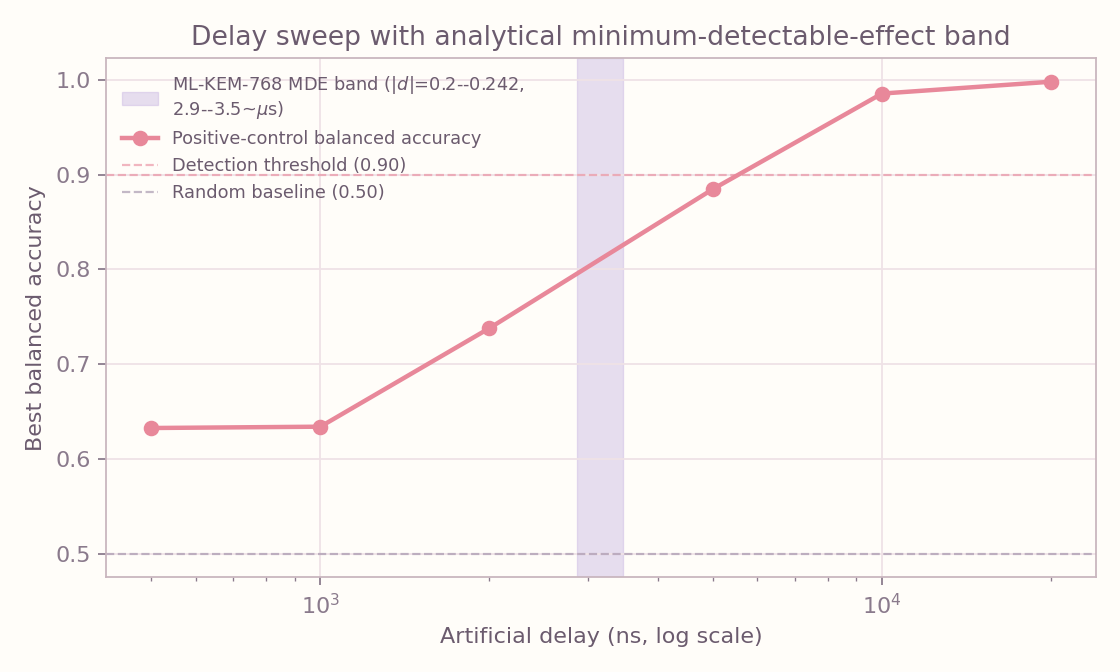
\includegraphics[width=0.78\textwidth]{delay_sweep_mde.png}
  \caption{延迟扫描曲线与 ML-KEM-768 最小可检测效应（MDE）区间的叠加。}
  \label{fig:sweep_mde}
\end{figure}

因此，本文真实场景"未检测到泄漏"的结论可更精确地表述为：在逐轨迹近似独立、每类
$n=400$、$\alpha=0.01$ 的假设下，本文对大约2.4--3.5~$\mu$s（视参数集而定）的稳定
均值差异具有约80\%检出功效。由于这些聚合样本来自60个基础密文组，且本文未执行严格的
等效性检验，上述功效分析不能被解释为对该量级以下或以上差异的形式化排除；量级更小、
更依赖组结构或只出现在特定输入子空间的潜在差异仍不在本文方法的可分辨范围内。

\subsection{特征重要性与运行稳定性}

图~\ref{fig:features} 展示了 \texttt{single\_bit} 策略下随机森林特征重要性在三个
参数集之间的比较。各特征重要性整体较为分散，没有出现单一特征在真实场景中稳定
主导分类的现象。这与模型准确率接近随机的结果一致：模型并未找到可泛化的泄漏方向。

\begin{figure}[H]
  \centering
  \includegraphics[width=0.86\textwidth]{variant_feature_importance.png}
  \caption{\texttt{single\_bit} 策略下三个参数集的随机森林特征重要性。}
  \label{fig:features}
\end{figure}

图~\ref{fig:stability} 给出60次实验的时间差稳定性。真实场景中的差异围绕0上下波动，
没有持续同向偏移；正对照场景则保持在接近20,000~ns 的正向差异附近，说明真实场景
中的小幅波动更可能来自操作系统调度、缓存状态和测量噪声，而不是稳定输入相关信号。

\begin{figure}[H]
  \centering
  \includegraphics[width=0.98\textwidth]{run_stability.png}
  \caption{60次实验中真实场景与正对照场景的平均时间差稳定性。}
  \label{fig:stability}
\end{figure}

\section{讨论}
\label{sec:discussion}

\subsection{结果解释}

统计检验、效应量和机器学习结果共同支持同一结论：在本文设置下，未检测到
\texttt{pqcrypto} ML-KEM 解封装实现对有效密文和四类无效密文表现出稳定、可利用的
时间差异。尤其需要注意的是，真实场景的最佳模型准确率最高单次仅0.5566，虽偶有
高于0.5的结果，但跨轮次、跨参数集和跨策略后均不稳定，也没有同时满足统计显著性与
效应量阈值。正对照的高准确率说明这一负结果不能简单归因于检测程序失效。

从数据本身看，实验结果更像是噪声条件下的弱随机波动，而不是采集失败或明显泄漏。
60次真实场景中，仅1次最佳平衡准确率超过0.55，且没有任何一次超过0.60；Welch's
$t$ 检验只有2次低于0.05，没有一次低于0.01；Cohen's $d$ 的绝对值最大为0.1501，
低于本文设定的小效应阈值0.2。平均时间差的方向也不稳定，跨实验最小值为
-1691.5~ns，最大值为2014.8~ns，说明单次均值差异容易受到操作系统调度和运行状态
影响。与之相对，正对照最佳平衡准确率均值达到0.9995，说明当时间信号足够强时，
本文流程能够稳定识别。因此，本文结果应被表述为有边界的负检测结果，而不是算法或
实现的形式化安全证明。

需要强调的是，本文的负检测结果并不意味着检测流程缺乏灵敏度。固定延迟正对照在全部
实验中均能被稳定识别，延迟灵敏度扫描也显示，当人为延迟达到一定量级时，统计检验、
效应量和机器学习分类会同时给出明确响应。因此，真实场景未触发泄漏判定，更合理的
解释是在当前软件计时条件和输入模型下，被测实现没有表现出超过检测阈值的稳定时间
差异。

ML-KEM-512、ML-KEM-768 和 ML-KEM-1024 的平均解封装时间随参数增大而增加，
\texttt{single\_bit} 策略下有效密文5轮均值约为28.25~$\mu$s、41.96~$\mu$s 和
60.12~$\mu$s。但计算量增长并未带来更明显的有效/无效分类信号，说明在所测实现和
输入模型下，参数集变化主要影响整体耗时，而不产生稳定标签相关差异。

\subsection{实验局限性}

本文结论具有明确边界。首先，软件计时在通用操作系统上不可避免地受到任务调度、
动态频率、缓存状态和后台 I/O 的影响。聚合重复、预热和随机打乱只能降低噪声，不能
等同于硬件实验台的隔离测量。其次，本文标签区分的是有效密文与无效密文，而不是
私钥比特或秘密中间值；即便检测到差异，也仍需进一步分析其是否可转化为密钥恢复
攻击。第三，实验对象限定为 \texttt{pqcrypto==0.3.4} 的具体绑定，不能直接推广至
所有 ML-KEM 实现、所有编译器选项或所有处理器平台。最后，本文只测试四类无效密文
模型，不能覆盖所有选择密文输入空间。

关于平台局限性，项目早期还在 macOS arm64（Apple Silicon）平台上对 ML-KEM-768 进行
过5轮探索性实验，作为本文正式实验之外的补充观察。该探索性实验在方法学上与本文
正式流水线存在差异：每类样本数为240（而非400）、每条聚合轨迹重复35次（而非50
次）、特征维度为9维（而非13维）、分类器仅包含线性 SVM 和随机森林两种（而非四种），
且运行环境为 Python 3.9.6。在这一不同处理器架构和不同流水线参数下，5轮真实场景
结果同样均未触发泄漏判定（最佳模型平衡准确率0.448--0.525，Welch's $t$ 检验
$p$ 值介于0.071--0.617之间），而正对照在5轮中均能被稳定识别（平衡准确率均不低于
0.99，时间差均接近20,000~ns）。表~\ref{tab:macos}列出了5轮的详细结果。该探索性
结果在定性层面与本文 Windows x86\_64 上的正式结论一致，但由于样本量、特征集和
模型集均不同，不构成严格的跨平台对照实验，仅作为本文方法在 x86\_64/arm64 与
Windows/macOS 之间定性可复现性的初步佐证；逐一参数集/策略组合的严格跨平台矩阵
留作后续工作。

\begin{table}[H]
  \centering
  \caption{macOS arm64 探索性实验（ML-KEM-768，5轮）}
  \label{tab:macos}
  \begin{tabular}{rrrrrr}
    \toprule
    轮次 & \multicolumn{3}{c}{真实场景} & \multicolumn{2}{c}{正对照} \\
    \cmidrule(lr){2-4} \cmidrule(lr){5-6}
     & 最佳平衡准确率 & Welch $p$ & Cohen's $d$ & 最佳平衡准确率 & 时间差（ns） \\
    \midrule
    1 & 0.525 & 0.071 & -0.165 & 0.993 & 21355.2 \\
    2 & 0.511 & 0.173 & 0.125  & 1.000 & 20132.0 \\
    3 & 0.503 & 0.256 & -0.104 & 1.000 & 20516.5 \\
    4 & 0.515 & 0.552 & -0.054 & 1.000 & 20253.3 \\
    5 & 0.512 & 0.617 & 0.046  & 1.000 & 20555.7 \\
    \bottomrule
  \end{tabular}
\end{table}

此外，本文的观测粒度是端到端解封装耗时，而 KyberSlash 等工作揭示的密钥相关时序
泄漏可能来自单条变长除法或压缩指令，其耗时差异在纳秒级总时间中可能被其他噪声源
淹没~\cite{Bernstein2025}。因此，本文的负结果不能说明被测实现在指令级别不存在
此类问题，只能说明在端到端黑盒计时这一观测粒度下未发现稳定可区分信号；若要排查
KyberSlash 类问题，需要结合源码审计或指令级污点分析等更细粒度的方法。

\subsection{可复现性与后续工作}

项目保留了完整采集脚本、原始 CSV、JSON 分析报告、数据质量报告和论文图表。后续
工作可以从三个方向展开：第一，在 Linux x86\_64、macOS arm64 和不同 CPU 微架构上
重复完整矩阵，比较平台差异；第二，使用更高重复次数或进程绑定、性能模式锁定等
方法降低软件计时噪声；第三，将同样的输入模型扩展到功耗或电磁轨迹，比较软件时序
与物理侧信道的灵敏度差异。

为支持独立复现，本文采集脚本、原始计时 CSV、统计与机器学习分析的 JSON 报告、
数据质量报告以及生成本文全部图表的代码均随项目一并提供，具体目录结构和重新运行
命令见附录。第三方可在安装相同版本依赖后，直接基于附录中的命令重新生成本文主要表图，
包括表~\ref{tab:matrix}--\ref{tab:mde}和图~\ref{fig:all_dist}--\ref{fig:stability}
中的全部结果。

\section{结论}
\label{sec:conclusion}

本文围绕 ML-KEM 解封装实现，建立了一套结合统计检验、机器学习分类和正对照验证的
软件时间侧信道泄漏筛查框架。该框架能够从均值差异、分布差异、效应量和多维特征
可分性等多个角度评估有效密文与无效密文之间是否存在稳定时间信号。

实验覆盖 ML-KEM-512、ML-KEM-768 和 ML-KEM-1024 三个参数集，以及四类同长度无效
密文策略。结果显示，60次真实场景实验均未触发泄漏判定，最佳模型平衡准确率接近
随机基线，Cohen's $d$ 未达到小效应阈值，统计检验也未形成稳定显著模式。与此同时，
固定延迟正对照能够被稳定识别，说明检测管线具备发现已知时间信号的能力。

因此，本文得出谨慎结论：在当前 Windows 11 x86\_64 软件计时条件、\texttt{pqcrypto}
版本和本文测试的输入模型下，未检测到 ML-KEM 解封装实现对有效密文与无效密文表现出
稳定、可区分的时间侧信道泄漏。该结论属于实现级筛查结论，不构成形式化侧信道安全
证明，也不能替代跨平台实验、硬件性能计数器分析、功耗分析或电磁侧信道评估。

\clearpage
\phantomsection
\addcontentsline{toc}{section}{参考文献}
\bibliographystyle{plain}
\bibliography{references}

\clearpage
\appendix
\phantomsection
\addcontentsline{toc}{section}{附录}

\section*{附录}

\subsection*{实验复现命令}

本文实验代码已保存在项目目录中。完整实验可在安装依赖后通过如下命令运行：

\begin{verbatim}
python -m pip install -r requirements.txt
python -m pip install -r requirements-dev.txt
python -m pip install -e .
export LOKY_MAX_CPU_COUNT=8
export MLKEM_PERMUTATIONS=20
bash scripts/run_paper_experiments.sh
\end{verbatim}

其中，\texttt{MLKEM\_PERMUTATIONS} 只影响输出报告中的置换检验辅助诊断，不参与正文
泄漏判定规则；若需要更精细的置换检验 $p$ 值，可提高该参数并重新运行分析。

若只需快速检查环境，可使用小规模冒烟测试：

\begin{verbatim}
RUNS=1 SAMPLES_PER_CLASS=20 REPETITIONS=5 N_GROUPS=5 \
VARIANTS="768" INVALID_STRATEGIES="single_bit" \
MLKEM_PERMUTATIONS=5 bash scripts/run_paper_experiments.sh
\end{verbatim}

\subsection*{主要数据文件说明}

\begin{table}[H]
  \centering
  \caption{论文实验相关输出文件}
  \begin{tabular}{>{\raggedright\arraybackslash}p{0.48\textwidth}
                  >{\raggedright\arraybackslash}p{0.42\textwidth}}
    \toprule
    路径 & 说明 \\
    \midrule
    \path{results/paper_runs/} & 5轮完整实验的原始 CSV 与 JSON 分析结果 \\
    \path{results/paper_artifacts/} & 论文图表与数据质量报告 \\
    \path{results/paper_artifacts/DATA_QUALITY_REPORT.md}
      & 标签平衡、缺失值、正对照有效性等检查结果 \\
    \path{summary.json} & 每个参数集/策略组合的统计检验和模型结果 \\
    \bottomrule
  \end{tabular}
\end{table}

\subsection*{泄漏判定规则}

本文采用保守的联合判定方式。真实场景只有在以下三个条件同时满足时，才报告检测到
时间泄漏：最佳模型平衡准确率不低于0.65；Welch's $t$ 检验 $p<0.01$；Cohen's
$d$ 的绝对值不低于0.2。正对照要求最佳模型平衡准确率不低于0.90，且 Welch's
$t$ 检验 $p<0.001$。这一规则用于避免单一统计量偶然显著导致误判。

\end{document}
